\chapter{Current State and Problems of CosmoScout}\label{ch:current-state/problems-of-cosmoscout}


\section{CosmoScout Concepts}\label{sec:cosmoscout-concepts}
\subsection{Control Scheme}\label{subsec:control-scheme}
\subsection{SPICE Coordinate Systems}\label{subsec:spice-coordinate-systems}


\section{Identified Problems}\label{sec:identified-problems}

In order to improve usability and reduce cybersickness symptoms, we aimed to identify and improve aspects and
scenarios in CosmoScout VR that led to cybersickness symptoms or general feeling of discomfort.
To identify these problems, we conducted small tests gathering empirical data, and used small interviews and
discussions with other developers and users of CosmoScout.
A formal study with unbiased test subjects was not done for several reasons, mainly since the goal is only vaguely
defined and may require a decently sized sample size, as well as time to process its results.
Additionally, the health and safety regulations and lockdowns around the COVID-19 outbreak complicated the feasibility
of any preliminary study.
The empirical data and interviews identified two major problem areas that need independent solutions to mitigate
discomfort and sickness symptoms.
The 6-Degrees-of-Freedom (6-DOF) in interplanetary space can easily lead to visually induced motion sickness, and the
rotations and translations of automatic navigation similarly have a tendency to lead to motion sickness symptoms,
especially the descending and ascending animations to navigate to a body's surface.


\subsection{Problems with free movement}\label{subsec:problems-with-free-movement}

While traditional 4-DOF-navigation provides an inherently more stable frame of reference with the fixed plane of
movement usually providing an up-direction strongly tied to the movement scheme, a 6-DOF-navigational system lacks this
reference frame as it allows the user to freely rotate around all axes.
A reference to the different degrees of freedom is shown in figure~\ref{fig:6-dof-reference}
\begin{figure}[h]
    \centering
    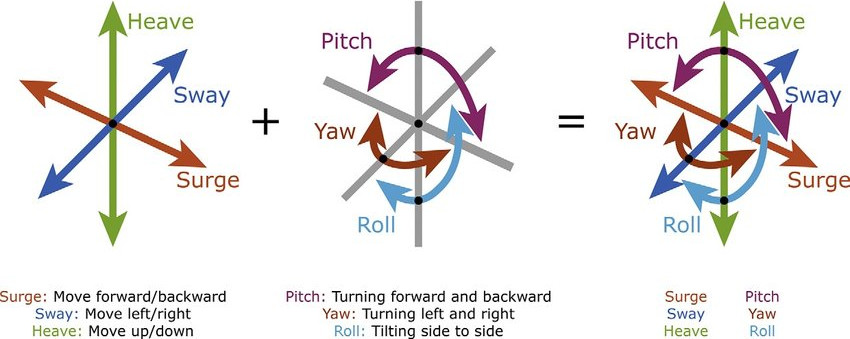
\includegraphics[width=\textwidth*2/3]{content/3_problems/img/6-DOF-reference[Fragaszy2018]}
    \caption{Six potential degrees of freedom for rotation and translation of a object~\cite{Fragaszy2018}.}
    \label{fig:6-dof-reference}
\end{figure}
Keshavarz, and Hecht~\cite{Keshavarz2011b} examined the influence of rotations around multiple axes and found that
increasingly complex rotations lead to an increase in cybersickness symptoms.
Additionally, Rebenitsch et al.~\cite{Rebenitsch2016} found multiple studies examining the effects of different
degrees of freedom in navigation.
They mention 6-DOF navigation usually induce more cybersickness symptoms than navigation with limited degrees of
freedom and conclude that the reason might be a limitation of rotation axes.
The control scheme of CosmoScout VR as described in section~\ref{subsec:control-scheme} does not allow for easy and
independent control of rotation around each axis, which can quickly lead to complex rotations around multiple axes at
once.
These complex rotations paired with a lack of reference frame can easily disorient the user and lead to visually
induced motion sickness symptoms.
While it seems both problems originate from the control scheme, a change of the control scheme does not necessarily
help mitigate the problems as different control schemes like those proposed by Drogemuller et al.~\cite{Drogemuller2020}
either suffer from the same problems, or significantly change the interaction context.
Isolating the rotation controls would be hard to implement with only the VR remotes and lead to a more unintuitive
and inconvenient control scheme.
Therefor, other mitigation methods are sought to provide the user with a stable frame of reference and reduce the
impact of complex rotations.


\subsection{Problems with automatic movement}\label{subsec:problems-with-automatic-movement}
